\chapter{\IfLanguageName{dutch}{Stand van zaken}{State of the art}}
\label{ch:stand-van-zaken}

% Tip: Begin elk hoofdstuk met een paragraaf inleiding die beschrijft hoe
% dit hoofdstuk past binnen het geheel van de bachelorproef. Geef in het
% bijzonder aan wat de link is met het vorige en volgende hoofdstuk.

% Pas na deze inleidende paragraaf komt de eerste sectiehoofding.

In deze stand van zaken zal verduidelijkt worden wat de hedendaagse problemen en bezorgdheden zijn in de wereld van de mainframe. Aan de hand van een literatuurstudie worden de problemen in kaart gebracht. 

\section{\IfLanguageName{dutch}{Het verdwijnen van expertise}{Lostage of expertise}}
\label{sec:Verdwijnen van expertise}

Veel informatietechnolgie specialisten, zoals Stewart Alsop voorspelden dat de stekker uit de mainframe zou worden gehaald aan het einde van de jaren 90 \autocite{McCracken2012}. Volgens het onderzoek van \textcite{Waites2013} zal de mainframe nog niet verdwijnen. Daarentegen verdwijnt de expertise wel. Mainframe-applicaties die kritisch zijn voor de werking van bedrijfsprocessen zorgen voor een angst dat de complexe expertise voor het ontwikkelen en onderhouden van deze applicaties aan het verdwijnen is. De mainframe-ontwikkelaars die geboren zijn tussen 1945 en 1964 zijn al gepensioneerd of gaan op pensioen. Dayton Semerjian, een senior vice-president bij CA Technologies zei ''The average age of mainframe workers is 55 to 60''. De grootste mainframeproducent, naast IBM, is CA Technologies. Veel organisaties zien outsourcing van hun workloads als een oplossing voor de tekorten van experten. Dit is een manier waarop ze een compensatie proberen te creeëren om hun mainframe workloads te behouden, doch tegelijkertijd te onderhouden en verbeteren. Het problematisch aspect hierbij is dat het heel tijdrovend en vermoeiend is voor een organisatie om de benodigde kennis door te geven. Aan de hand van technische kennis kan je bij mainframe-ontwikkeling heel wat doen, echter is kennis over de organisatie eveneens van groot belang.

Sinds 1960, het jaar dat dr. Grace Hopper en haar collega's COBOL hebben gecreëerd. Deze programmeertaal is naar schatting gegroeid van 150 tot 250 miljard lijnen applicatiecode, waarvan acht tot negen miljoen nieuwe lijnen per jaar worden bijgeschreven. Het is nog steeds de populairste programmeertaal in de mainframewereld. Anderzijds met de ontwikkeling van andere programmeertalen, wordt COBOL afgeschreven als 'out-of-date' en 'dying'. Elk jaar sinds 1970 werd het uitsterven van COBOL een volkomen zekerheid. Als een organisatie een mainframe heeft, zijn de kansen zeer groot dat al hun applicaties geschreven zijn in COBOL. Programmeurs die in de jaren 70 en 80 in de technologiesector instapten, was het heel waarschijnlijk dat zij een COBOL programmeur werden. Daarom is het duidelijk dat de leeftijd van mainframe-experten verschillend is van de leeftijddistributies die in de UNIX en Windows omgevingen plaatsvindt \autocite{McGirr}. Volgens studies van Meta Group zijn 60\% van de mensen die werken op een mainframeomgeving  50 jaar of ouder in vergelijking met de 8\% in een UNIX- of Windowsomgeving. Slechts vijf procent zijn onder de 30 jaar. Het is hieruit duidelijk te concluderen dat veel mainframe-experten de pensioenleeftijd aan het naderen zijn. 

In het verleden werden veel IT professionals geïntroduceerd in de informaticasector door te programmeren. Veel universiteiten boden COBOL cursussen aan in mainframeomgevingen. Met het opkomen van nieuwe en modernere programmeertalen begonnen universiteiten deze cursussen uit te dunnen of zelfs te schrappen uit hun curriculum. Hierdoor verloor de programmeertaal COBOL zijn populariteit. Studenten voelden zich meer aangetrokken tot de meer moderne en aantrekkelijke programmeertalen zoals Java en C++. Veel jonge IT professionals zien het niet meer zitten om op mainframesystemen te werken \autocite{Mullins2016}. De vraag is natuurlijk of we het ze kwalijk kunnen nemen. Het groene 3270 terminalvenstertje is niet het meest aantrekkelijke in vergelijking met de omgevingen zoals Eclipse, Visual Studio en Visual Studio Code. Wat de meeste onder de jonge IT professionals niet weten is dat het niet meer de norm is om enkel in dat groene terminalvenstertje te werken. De moderne mainframe is heel verschillend ten opzichte van wat de meeste studenten of IT professionals denken. Mainframes kunnen vandaag de dag gemakkelijk gekoppeld worden via de parallel sysplex technologie. Dit is een clusteringtechnologie die toelaat om verschillende kopieën te hebben van het Z/OS besturingssysteem in één enkele image. De tec

Deze technologie biedt de mogelijkheid om meerdere systemen te laten werken en toch hun data over alle systemen te kunnen raadplegen en gebruiken \autocite{Sarkar2020}. Daarnaast is het ook mogelijk om moderne technologieën zoals Linux- en Windowsplatformen te gebruiken op een mainframe. Dit wil zeggen dat je Java, XML, TCP/IP enzovoort kan gebruiken. De oorzaak van deze ontwetendheid is het gebrek aan kennis en het opleidingsaanbod. Mainframetechnologie wordt niet meer aangeleerd door universiteiten en/of hogescholen, dit zou moeten veranderen, maar zal het veranderen? We zouden de naam van de mainframe wat aantrekkelijker kunnen maken om ervoor te zorgen dat deze technologie terug aantrekkelijk wordt bij de nieuwe generatie IT professionals. \textcite{Mullins2016} vond de naam AlwaysAvailable een passende naam.


Volgens een online artikel van Open Mainframe Project \autocite{2020}, zijn er 4300 instellingen in de Verenigde Staten waar het mogelijk is om een diploma te verkrijgen. Slechts 10 tot 15 instellingen bieden een semestriele cursus aan dat te maken heeft met mainframe. De reden die zij hiervoor beschouwen is het feit dat er een tekort is aan facultatieve kennis om deze cursussen aan te bieden. Mainframe-experten zouden hun kennis opgedaan hebben on the job en niet meer via hun opleiding. Dit zorgt ervoor dat deze personen niet toegelaten worden om hun kennis door te geven op academisch niveau. 

\section{\IfLanguageName{dutch}{De laatste nieuwe mainframe technologie}{The most recent mainframe technology}}
\label{sec:De laatste nieuwe mainframe technologie}

Er wordt wel eens vaak gezegd dat de mainframe dood is. De mainframe is over de jaren heen al zoveel keren dood verklaard. Toch wordt de 'Big Iron' gemoderniseerd en nog geen klein beetje. De nieuwste generatie mainframe van IBM heeft bewezen dat de mainframe nog sterk aan innovatie onderheven is \autocite{Almekinders2022}. Volgens IBM zullen mainframes nog zeker deel uitmaken van de hedendaagse informatica en dat hebben ze bewezen door hun introductie van de IBM Z16. Deze nieuwe mainframe bevat een Telum-processor. Hierop bevindt zich een accelerator met AI-inferencing. Dergelijke systemen bieden klanten tijdige, geïnformeerde en aangepaste oplossingen om beslissingen te helpen maken, terwijl ze tegelijkertijd geschikte beveiligingsmechanismen voor AI-modellen gebruiken \autocite{Cammarota2020}. In het geval van de Z16 beloofd IBM dat dit realtime AI toevoegt aan workloads die op een dergelijke mainframe gedaan worden. Via de Telum processor kunnen banken fraude gaan detecteren tijdens transacties op grote schaal. Als gevolg hiervan kan voorkomen worden dat klanten en/of bedrijven grote verliezen maken vanwege frauduleuze praktijken. De Z16 mainframe kan met behulp van artificiële intelligentie ervoor zorgen dat de kans op fraude significant wordt verkleind. Fraude zou opgemerkt en gesignaliseerd kunnen worden, nog voor de transactie volbracht is \autocite{Saran2022}. Hiermee zetten zij in op maximale security van transacties. Dit zonder impact op de SLA's(Service Level Agreements). Een service level agreement of SLA definieert het servicelevel dat door de klant wordt verwacht van de fabricant of leverancier van een dienst of product. Volgens bepaalde criteria wordt een doelstelling van tevredenheid over het dienst of product vastgelegd waar dan een akkoord wordt over gesloten. Zo wordt van de nieuwe mainframe verwacht dat pure prestatie worden behouden om aan de verwachtingen van hun klanten te kunnen voldoen. Banken en verzekeringsinstellingen kunnen dezelfde latency verwachten, echter met artificiële intelligentie er bovenop. AI-inferencing maakt het mogelijke voor financiële instellingen om transacties sneller en efficiënter af te handelen. Een praktisch voorbeeld waarbij AI-inferencing nuttig kan zijn is het versnellen van de afsluitingen van leningen en het bepalen van welke transacties hogere risico's met zich meebrengen.


\subsection{\IfLanguageName{dutch}{Quantum computing en IBM Z16}{Quanting computing and IBM Z16}}
\label{sec:Quantum computing en IBM Z16}

IBM speelt een ontzettend grote rol in de wereld van quantum computing. De ontwikkeling van deze vrij nieuwe technologie heeft ook een donkere zijde. Veel cryptografiemethodes kunnen eenvoudig worden doorbroken door quantum gebaseerde gevallen. Denk hierbij maar aan het uitwisselen van walletkeys of digitale handtekeningen. De wiskundige methodes die deze zaken gebruiken zijn eenvoudig op te lossen met een quantumcomputer. Volgens Anne Dames, Distinguished Engineer, Cryptographic Technology Development Systems bij IBM wordt het aanvalsoppervlak van systemen en organisaties met quantum computing een stuk vergroot \autocite{Almekinders2022}. Natuurlijk moet de IBM Z16 dit probleem tegengaan. De nieuwe mainframe maakt gebruik van lattice-based cryptografie. Hiermee is het mogelijk om wiskundige probleemstellingen te creëren die zelfs quantumcomputers niet kunnen oplossen. 

\section{\IfLanguageName{dutch}{IBM Mainframe modernisatie}{IBM Mainframe modernization}}
\label{sec:IBM Mainframe modernisatie}


\subsection{\IfLanguageName{dutch}{Workloads migreren naar de cloud - Google Cloud Platform}{Migrating workloads to the cloud - Google Cloud Platform}}
\label{sec:Workloads migreren naar de cloud}


Google Cloud is een uitstekende keuze als het gaat om een omgeving waar een IBM z/OS mainframe workload naar zou kunnen gemigreerd worden \autocite{Astadia2021}. Dit platform biedt gelijkaardige securitylevels en de mogelijkheid om te kunnen schalen naar wat de gebruiker ervan verwacht. Het biedt enerzijds ook een omgeving die z/OS mainframe legacy ondersteund dat is gemigreerd naar de cloud. Volgens \textcite{Astadia2021} zijn het aantal personen die de skills beheersen om mainframe legacy te onderhouden aan het dalen en worden zij niet vervangen. Anderzijds stijgen hardware- en softwareonderhoudskosten continue om te kunnen voldoen aan de innovatieve eisen die vele klanten hebben. Innoovatieve eisen die IBM z/OS mainframe platformen niet kunnen bieden. 

\subsection{\IfLanguageName{dutch}{Wat is Astadia?}{What is Astadia?}}
\label{sec:Wat is Astadia?}

Sinds 1994 is Astania één van de grootste uitdagingen op vlak van modernisatie, cloudmigratie, replatformering en applicatiemodernisatie aangegaan in het hedendaagse bedrijfsleven. Zij zijn wereldleider in high-performance mainframe modernization. Zij helpen organisaties om een transformatie roadmap op te stellen om weg te migreren van hun mainframe legacy. 

\subsection{\IfLanguageName{dutch}{Waarom zouden we onze mainframe legacy en databases migreren naar Google Cloud?}{Why should we migrate our mainframe legacy and databases to Google Cloud?}}
\label{sec:Waarom zouden we onze mainframe legacy en databases migreren naar Google Cloud?}

Volgens Astadia is het kostenplaatste al een interessante factor om een migratie te overwegen. De TCO (Total Cost of Ownership) van een platform zoals Google Cloud versus IBM z/OS mainframe zou op een kortetermijn van 12 maanden al een aantrekkelijke ROI (Return On Investment) geven. Daarnaast beweren zij ook zoals in de voorgaande alinea's van het onderzoek dat de mensen die de juiste skills bevatten aan het verminderen zijn en niet vervangen worden. Het aanbod van IT professionals met de nodige kennis en expertise verdwijnt \autocite{Astadia2021}. Google Cloud daarentegen is een aantrekkelijker en meer populair platform dat wereldwijd meer jonge IT professionals naar zicht toe trekt. Ten slotte speelt de flexibiliteit volgens Astadia een grote rol. Volgens hun is Google Cloud meer flexibel op vlak van het schalen van businessvereisten. Het ondersteunen van grote aantallen gebruikers en toestellen zou beter tot zijn recht komen, net als database sharing. 

We spreken in dit onderzoek vaak van moderniseren of migreren. Migreren is eigenlijk een type van modernisatie. Migratie houdt natuurlijk ook andere zaken in zoals replatform, refactor, rewrite en replace processen. Laat ons beginnen met wat we begrijpen onder replatform. Dit is een proces dat bestaande code hetzij in COBOL, hetzij in PL/1 gaat van de mainframe halen. Deze code zal dan gecompileerd en gedraaid worden in een z/OS emulator die draait op Google Cloud. Dit is een manier om tijd en geld te besparen. Indien alle bestaande legacy code moet herschreven worden kost dat veel tijd en de juiste mensen om dat te verwezenlijken. IBM z/OS applicatie gaan draaien op een gehoste emulator door Google Cloud brengt de mogelijkheid met zich mee om API's te gaan voorzien voor eerder ontoegankelijke programma's en data. Vaak is het wel zo dat mainframeapplicatiecode eerder worden omgevormd naar Java of C\#. Deze programmeertalen zijn object georiënteerd wat beter past bij de aard van cloud-gebaseerde applicaties. Dit staat bekend onder het proces refactor. Natuurlijk is de enige praktische en efficiënte manier om dit te doen , het proces automatiseren om mainframeapplicatiecode te transformeren. Als voorlaatste proces binnen een migratie naar de cloud heb je rewrite. Dit komt er op neer dat je nieuwe programma's gaat ontwikkelen om de IBM z/OS mainframe te gaan moderniseren. Vaak is dit riskant en het meeste van de pogingen om programma's te herschrijven mislukken. Het is te complex en het kostenplaatje dat er komt bij kijken is zeer hoog. Een betere aanpak is om de applicatie te verplaatsen naar een Google Cloud gebaseerde emulator. Dat houdt in dat er ook gemigreerd wordt naar een Google Cloud gebaseerde databank en dat de focus gelegd wordt op het vervangen van modules en code in verschillende fases. Als het tijd is om aan rewrite te gaan doen, zijn transformatie-engines vaak de beste optie die het risico zo laag mogelijk houden. Als laatste proces in de migratie naar Google Cloud hebben we het replace proces. De bedoeling hiervan is om de functionaliteit van de mainframe  te gaan vervangen door een programma of een verzameling van programma's. Dit is typsiche een Software-as-a-Service (SaaS) applicatie. 

\subsection{\IfLanguageName{dutch}{De uitdagingen van mainframemodernisatie volgens Astadia}{De challenges of mainframe modernization according to Astadia}}
\label{sec:De uitdagingen van mainframemodernisatie volgens Astadia}

In de informatie technologie en met name software development is het steeds aangewezen om documentatie over een bepaalde applicatie of stukje software bij te houden. Natuurlijk is dit niet altijd zo geweest. In de vroege jaren van commerciële mainframe computing werd dit nooit gedaan. De ontwikkelingen rond softwaredocumentatie begonnen rond deze tijd pas onder stoom te komen \autocite{Zachry2001}. Dit sluit dan ook meteen  bij de uitdagingen die volgens Astania op de weg liggen bij een mainframemodernisatie. Veel IBM z/OS mainframeomgevingen vertrouwen dagelijks op honderden applicaties en transacties waar geen documentatie voor bestaat waarin beschreven staat wat ze juist doen. In veel gevallen zijn applicaties op mainframe al een paar decennia oud. Daarnaast hebben veel van deze applicaties dependencies of afhankelijkheden binnen het systeem om hun taak te doen. Denk maar aan een DB2 databank of een groep van sequentiële bestanden. Als deze dependencies niet gedocumenteerd zijn is het moeilijk om te achterhalen wat deze applicaties nodig hebben tijdens hun uitvoering. Om een succesvolle migratie door te voeren is het van essentieel belang dat ook de dependencies mee gemigreerd worden met de applicatie. Anderzijds is er een uitdaging dat te maken heeft met het draaien van parallelle systemen. Bij sommige IBM z/OS mainframe applicaties is het nodige om aan parallelle verwerking te doen, terwijl deze applicatie nog steeds in gebruik is in de productieomgeving en tegelijk op het nieuwe platform. De planning en de uitvoering voor deze processen, is een uitdaging dat hoort bij de migratie van een IBM z/OS mainframesysteem. Ook moet er rekening worden gehouden met de integriteit van data. Bij het migreren van een grote databank naar een nieuwe doeldatabank vereist een reorganisatie en ordening van de oude data. Dit is nodig om de integriteit van data te bewaren. Hieruit kan geconcludeerd worden dat bij een migratie volgens Astadia het een goed moment is om een validatie uit te voeren van de organisatiedata \autocite{Astadia2021}. Het kostenplaatje is vaak een achilleshiel in de migratie van het IBM z/OS platform naar een Google Cloud omgeving. Organisaties hebben bij het moment van een migratie een dubbele kost die zij moeten betalen. Ze betalen voor het in stand houden van de productieomgeving die draait op een mainframe, terwijl zij alle moeite en geld steken in de migratie naar het nieuwe systeem. Dit heeft een tijdelijk financiële impact op de welvaart van een organisatie waar rekening moet mee gehouden worden. Ten slotte is de expertise tijdens een migratie van heel groot belang. Het is een vereiste dat er zowel expertise is op vlak van de organisatiestructuur als technische kennis van de nieuwe programmeertalen, databanksystemen, netwerken en vele andere componenten. Alle workloads die gemigreerd worden naar Google Cloud moeten dezelfde functionaliteit bewaren als voordien. Hierdoor is het belangrijk dat de functionele analisten binnen de migratieplannen een gedetailleerd ontwerp uittekenen die alle use cases in kaart brengen van de oude mainframeapplicaties. Door het iteratief en consistent uitvoeren van testen moet het doel zijn dat het Google Cloud platform werkt zoals het IBM z/OS mainframe platform. 

\subsection{\IfLanguageName{dutch}{De voordelen van migreren naar Google Cloud volgens Astadia}{De benefits of migrating to Google Cloud according to Astadia}}
\label{sec:De voordelen van migreren naar Google Cloud volgens Astadia}

Volgens \citeauthor{Astadia2021} is het makkelijker om te gebruiken dan het IBM z/OS mainframeplatform. Google Cloud is ontworpen met eenvoudigheid in het achterhoofd. Het is mogelijk om nieuwe services en applicaties te hosten door het gebruik van de ``web-based Google Cloud Management Console ``.  Er is veel meer documentatiebeschikbaar en online informatie op fora en websites. Het is daarnaast ook een flexibeler systeem, omdat het mogelijk is om een groot aantal virtuele omgevingen te kiezen die het best bij jouw workload passen en die overeenstemmen met de vereisten van de applicaties. In het geval dat er geen adequate omgeving wordt gevonden, kan er simpelweg een andere type van instantie worden voorzien. Google Cloud is beter op vlak van prijs/kwaliteit volgens \citeauthor{Astadia2021}. Er wordt enkel betaald voor de resources die gebruikt worden zonder vastliggende contracten of verplichtingen. Bij het gebruik van een IBM z/OS mainframesysteem hebben organisaties een hoge verwachting op vlak van betrouwbaarheid, veiligheid en snelheid. Google Cloud biedt een wereldwijde computerinfrastructuur die al deze factoren evenaart volgens \citeauthor{Astadia2021}. Google Cloud biedt daarnaast meerdere security capabilities en services  die privacy verbeteren. Deze omvatten Google Cloud Virtual Private Cloud(VPC), die private of dedicated netwerkconnecties encrypteerd. 

\subsection{\IfLanguageName{dutch}{Zijn IBM z/OS mainframeworkloads goede kandidaat voor migratie naar een publieke cloudomgeving?}{Are IBM z/OS mainframe workloads good candidats for migration to public cloud environment?}}
\label{sec:Welke workloads kunnen gemigreerd worden naar de cloud?}

Een publieke cloud is een platform dat gebruik maakt van een standaard cloud computing model om resources beschikbaar te stellen voor cloudcomputing \textcite{Allison2016}. Typische IBM z/OS mainframe workloads waaronder COBOL, PL1, CICS en IMS zijn geen geschikte workloads om naar een publieke cloudomgeving te migreren. De reden hiervoor is het besturingssysteemomgeving. De controle of een workload geschikt is gebeurt op basis van verschillende criteria. Veronderstel dat de workload wel een geschikte kandidaat is voor een migratie naar een cloudomgeving, dan is de volgende stap om na te denken over de opslaglagen. Een voorbeeld van een opslaglaag is de cloud, maar een workload heeft altijd meerdere lagen. Deze worden bepaald aan de hand van prestaties, I/O capaciteit, beschikbaarheid en schaalbaarheid \autocite{Allison2016}. Volgens het onderzoek van \citeauthor{Martikainen2018} zijn er geen duidelijke karakteristieken waar een mainframe workload moet aan voldoen om te migreren naar de cloud. Organisaties hebben verschillende soorten applicatiearchitecturen op hun mainframe. Daardoor variëert de complexiteit van de bestaande applicaties door de onderliggende architecturen. \citeauthor{Orban2016} stelt voor om hierover na te denken op basis van een spectrum van complexiteit. De gevirtualiseerde service-georiënteerde architectuur zou aan de lage complexiteit van het spectrum liggen en de monolitische mainframe aan de hoge complexiteit van het spectrum. Volgens hem zou het starten aan de lage complexiteit van het spectrum gemakkelijker te volbrengen zijn bij een migratie, waardoor de kans groter zou zijn op slagen \autocite{Orban2016}. 

Het is het beste om eerst te focussen op de minst complexe of strategische applicaties \autocite{Korzenlowski2017}. Dit zijn applicaties die gebruikers nodig hebben om hun werk te kunnen uitvoeren of die essentieel zijn voor de organisatie. Volgens het artikel van \citeauthor{Marble2017} zijn mainframeworkloads en architecturen uitermate complex. Het feit dat mainframes duizende transacties kunnen verwerken per seconde spreekt voor zich. Er is nood aan een perfecte planning om een mainframeworkloads te gaan migreren naar open systemen \autocite{Marble2017}. De eerste stap in een migratieplan is om te kijken naar elk aspect in de workload zoals: 
    \begin{itemize}
        \item Omgevingen
        \item Applicaties
        \item Databanken
        \item Packages
        \item Utilities
        \item Tests
        \item Gebruikers
        \item Programmeertalen
    \end{itemize}
Vervolgens moet je de focus leggen op het doel van de applicaties en de vereisten om een hiërarchische opstelling te kunnen maken op basis van de businesswaarde \autocite{Marble2017}. Hierna kan je een duidelijke visuele representatie maken  de applicaties binnen de mainframeworkload bij het ontwikkelen van het migratieplan. 
\begin{figure}
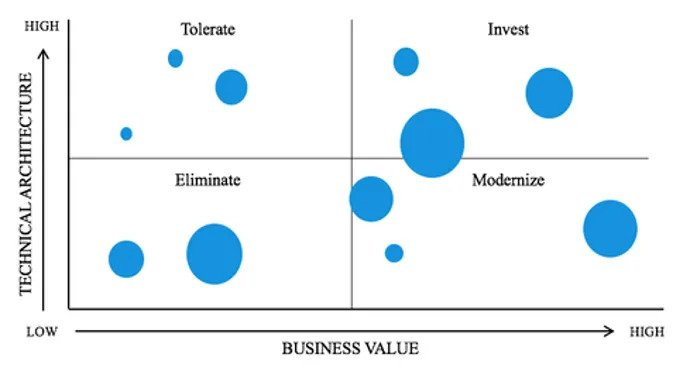
\includegraphics[width=12cm]{businessvalue}
\caption{Visuale representatie van businesswaarde voor mainframeapplicaties \autocite{Marble2017}}
\end{figure}

Op basis van dit model kan bepaald worden welke applicaties het eerst zouden kunnen gemigreerd worden. Daarnaast kan bepaald worden welke legacy applicaties er best wachten tot het einde van het migratieproject. 

\subsection{\IfLanguageName{dutch}{Workloads migreren naar de cloud - Microservices}{Migrating workloads to the cloud - Microservices}}
\label{sec:Workloads migreren naar de cloud}

Een service is het ophalen of publiceren van data aan een remote systeem \autocite{Linthicum2016}. Volgens \citeauthor{Linthicum2016} is een voorbeeld van een service het proces om een risicoanalyse te berekenen bij een financiële transactie. Dat is de fundamentele werking achter een service-oriented architecture (SOA). Microservices is echter ook een architectuur, maar wordt volgens \citeauthor{Linthicum2016} vaak verward met een SOA. Er is natuurlijk wel een bepaalde overlap in de twee technologieën. Het ontwerppatroon dat erachter zit werkt door applicaties die bestaan uit kleine processen die met elkaar communiceren door het gebruik van application programming interfaces (API)'s. De bedoeling bij service-oriented computing is dat applicaties worden gereduceerd tot enkel het functionele en die dan een set aan services aanbieden aan andere applicaties of de applicatie zelf. Het idee hierachter is het hergebruiken van functionaliteit \autocite{Linthicum2016}. 

Het gebruik van containers speelt bij microservices een grote rol. Met containers is het mogelijk om bestaande applicaties te gaan bundelen en de complexiteit te verlagen. Containers zorgen ervoor dat de applicaties niet meer afhankelijk zijn van hun onderliggende infrastructuurservices. Hierdoor is het mogelijk de toegang tot de opslag en resources loskoppelen van de applicaties en maakt dit de applicaties minder statisch \autocite{Linthicum2016a}. Microservices zijn net zo onafhankelijk en losgekoppeld. Het zijn geïsoleerde componenten die individueel kunnen gebruikt worden zonder effect op andere componenten. Het gebruik van Linux en/of Docker containers verzekeren dat services in dezelfde omgeving kunnen draaien in dezelfde omgeving \autocite{Bucchiarone2018}.

Volgens het rapport van \citeauthor{Bucchiarone2018} waarin de ervaring wordt beschreven van een migratie van een monolithisch systeem zoals mainframe naar Microservices, zal de mainframe voor lange tijd nog verbonden zijn aan de Microservice-technologie. Echter zal het mogelijk zijn om uiteindelijke de functionaliteiten van de mainframe te implementeren als nieuwe services. Dit zal resulteren in het definitief ontkoppelen van de mainframe \autocite{Bucchiarone2018}. 


\subsection{\IfLanguageName{dutch}{Workloads migreren naar de cloud - Amazon Web Services (AWS)}{Migrating workloads to the cloud - Amazon Web Services (AWS)}}
\label{sec:Workloads migreren naar de cloud}

\subsubsection{\IfLanguageName{dutch}{Het opzetten van een AWS Mainframe Modernizatie runtime omgeving)}{Deploying a AWS Mainframe Modernization Mainframe Modernization runtime environment}}
\label{sec:Het opzetten van een AWS Mainframe Modernizatie runtime omgeving}


